As shown earlier in Section \ref{sec:shufflealgos}, there are many alternatives for implementing distributed shuffle algorithms, of which some depend on performance characteristics of the underlying system.
Since in this paper, we want to use the NVIDIA NVSHMEM library for GPU-initiated network communication to build a GPU-initiated shuffle algorithms, we explore the performance characteristics of the networking primitives offered by the NVSHMEM library in this section. To build understanding we employ a benchmark strategy that tests specific functionalities or primitives in isolation, which is known as microbenchmarking \cite{kounev2020systems}.
Specific targets of this series of benchmarks are answering the questions:

\begin{itemize}
    \item (1) whether the tuples should be send out in larger batches,
    \item (2) if so, how large the batches should be, and
    \item (3) whether and how the sending can be parallelized.
\end{itemize}

All of the benchmarks have been carried out on two nodes connected with a 100 Gb/s Infiniband interconnect.

\begin{figure}[h]
    \centering
    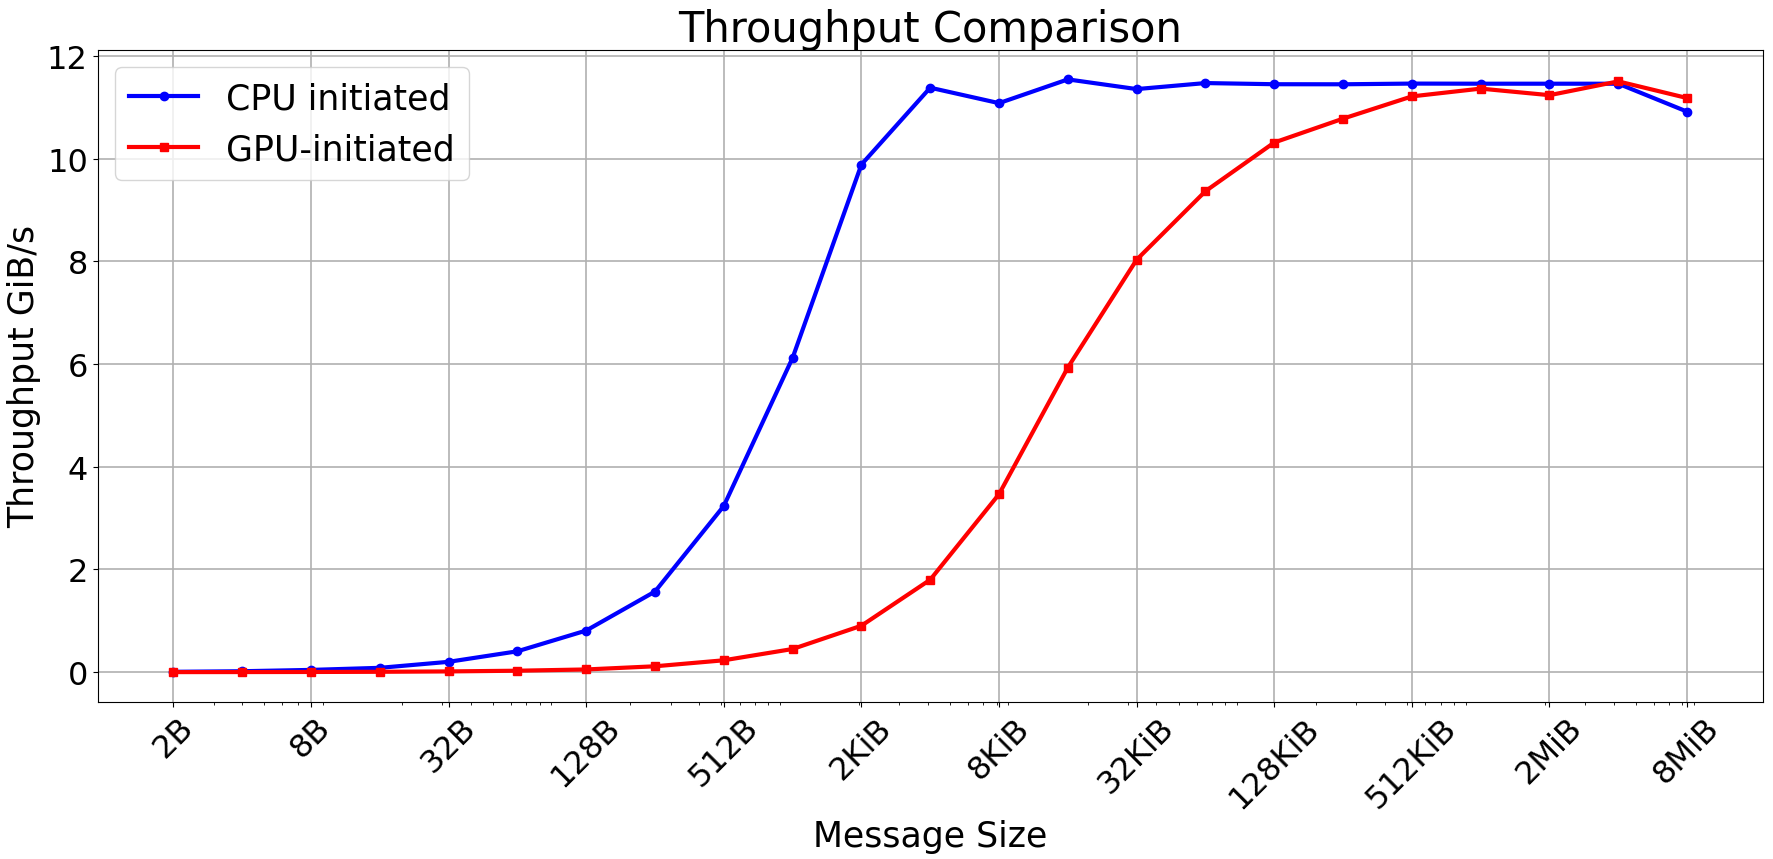
\includegraphics[width=0.7\textwidth]{img/09_gpu_cpu_st.png}
    \caption{Comparison of single-threaded CPU- and GPU-initiated networking performance based on the message size per send call}
    \label{fig:cpu_gpu_st}
\end{figure}

The first benchmark we conducted is visualized in Figure \ref{fig:cpu_gpu_st} and compares the throughput of CPU-initiated RDMA with GPUDirect (blue line) to GPU-initiated communication with NVSHMEM (red line).
In both scenarios, a single CPU thread (or GPU thread respectively) initiates a number of consectutive asynchronous RDMA operations with a certain message size per invocation.
Each invocation incurs some control flow overhead i.e. the instructions needed for asynchronously sending data, and metadata overhead i.e. the header of the messages sent to the NIC and over the network.
With smaller message sizes, the ratio between overhead and payload is greater.
Specifically the control flow overhead limits the throughput if it takes longer to initiate the asynchronous sending from the computing device than it takes from that point on to send the data to the destination.
Consequently, Figure \ref{fig:cpu_gpu_st} shows that larger message sizes increase the system's throughput up to the point where it is limited by the capacity of the physical link (12.5 GB/s).
Comparing the two curves, however, we can see that GPU-initiated communication requires larger message sizes per interface invocation to saturate the physical link limit.
We interpret this as a cause of the higher clock frequency, more powerful instruction set and difference in implementation of the CPU-initiated communication in comparison to the GPU-initiated run.
Thus, an efficient implementation of GPU-initiated shuffle would need to either use larger messages for sending or benefit from some other optimization to compete with a CPU-initiated reference implementation.
One of those optimizations could be a possible parallelization of the send calls across multiple GPU threads.

\begin{figure}[h]
    \centering
    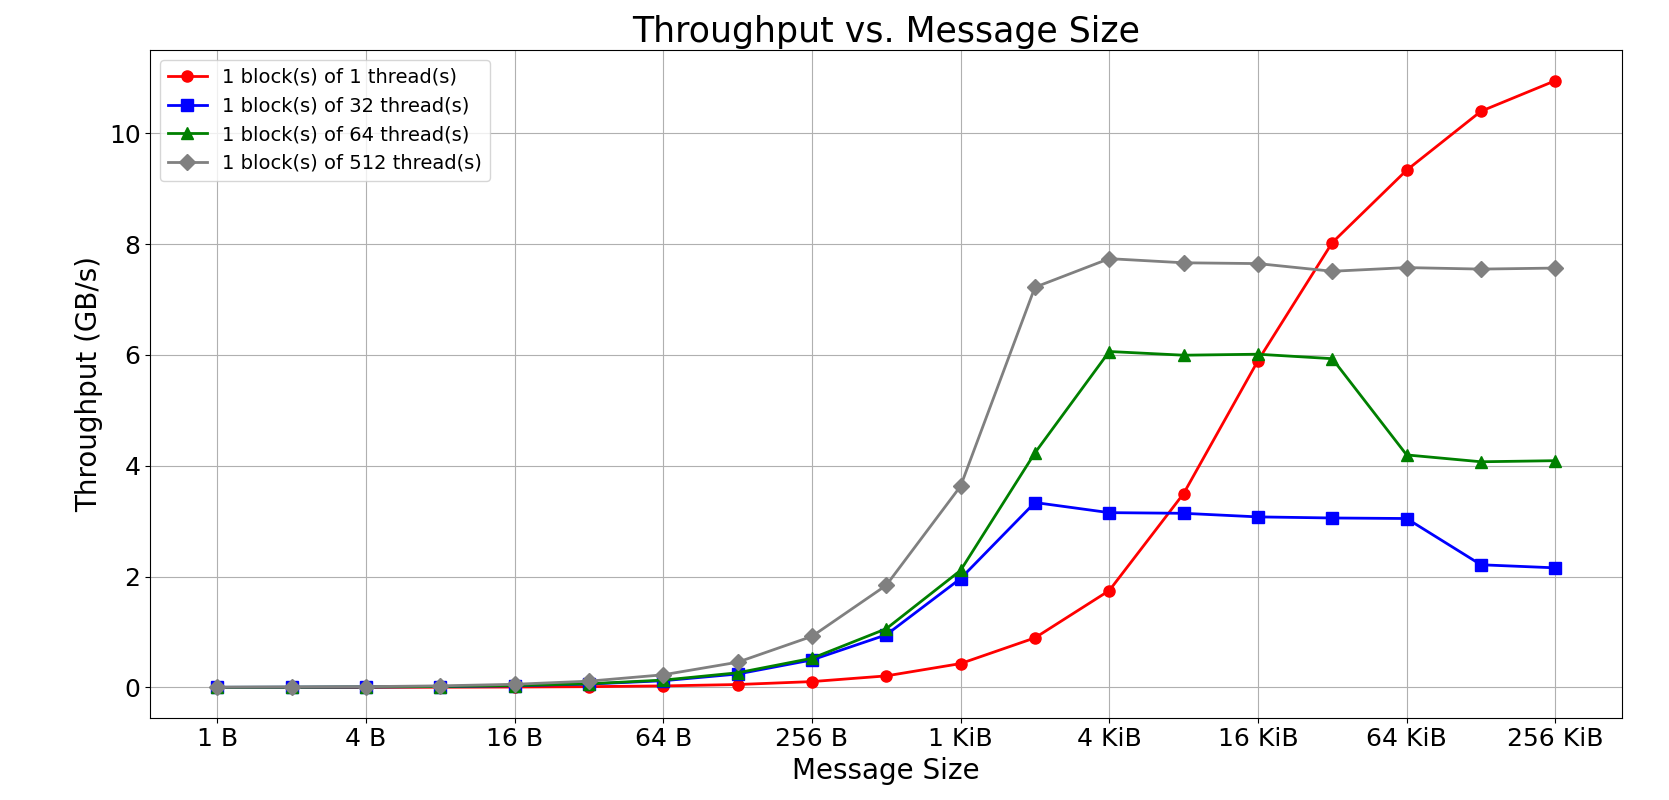
\includegraphics[width=0.8\textwidth]{img/put_granularity_grid1.png}
    \caption{Throughput for repeated nvshmem\_put\_nbi calls using one thread block}
    \label{fig:put_gran_grid_1}
\end{figure}

To analyze the parallelization of send operations in NVSHMEM, we have conducted another series of benchmark which is shown in Figure \ref{fig:put_gran_grid_1}.
These benchmarks use one GPU thread block with a different number of threads and send the messages of the respective size shown on the x-axis using the NVSHMEM asynchronous interface.
Since the read line uses one thread block with one thread, it is equivalent to the red line in the previous plot in Figure \ref{fig:cpu_gpu_st}.
The other lines, which show the results of multiple threads in one block sending the data, show very interesting results.
All of those configurations allow for a faster growth in throughput compared to the single-threaded benchmark depending on the message size.
According to the tested configurations, larger number of threads show this effect more clearly.
Approximately at 4KiB, however, all of the multi-threaded configurations seem to hit some kind of limiting performance factor.
We have not managed to find out the definite reason for this behaviour but are guessing it might be related to the maximum transmission unit (MTU) or a translation look-aside buffer (TLB) related issue.
Without having certainty about the reason for this behaviour, we can nevertheless conclude that using parallelization for sending across threads within a GPU block is not going to be a promising way for the shuffle to work efficiently.

\begin{figure}[h]
    \centering
    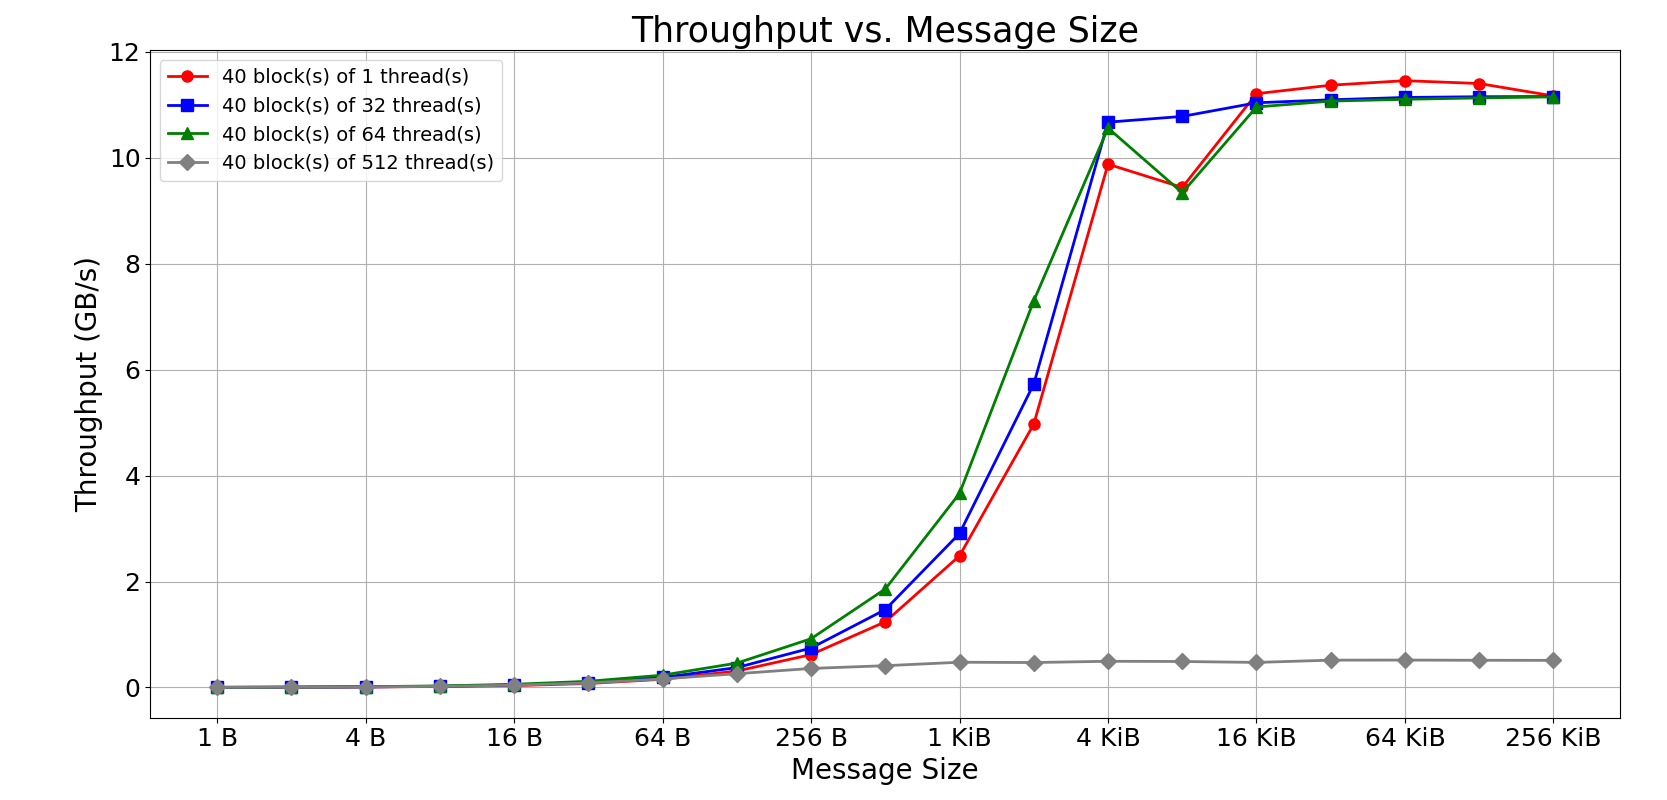
\includegraphics[width=0.8\textwidth]{img/put_granularity_grid40.png}
    \caption{Throughput for repeated nvshmem\_put\_nbi calls using 40 thread blocks}
    \label{fig:put_gran_grid_40}
\end{figure}

To explore other parallelization opportunities, we have run the benchmark again with a different configuration.
This time we are using 40 GPU blocks where each of the blocks includes a certain number of threads as shown in the legend of the plot.
Every of the $n_{threads} \cdot n_{blocks}$ threads in the system again sends messages using the NVSHMEM non-blocking interface.
Surprisingly, this plot shows very different results than the previous one.
Seemingly, the NVSHMEM implementation is not suitable for handling a number of threads as large as 20480 ($40$ blocks $\cdot$ $512$ threads), since the performance is extremely poor, as indicated by the grey line in Figure \ref{fig:put_gran_grid_40}.
On the other hand, all other configurations show very good results, that are comparable to those of CPU-initiated networking shown earlier in Figure \ref{fig:cpu_gpu_st}.
All configurations seem to stagnate just below the physical link bandwidth, which is a sign of good performance.
Nevertheless, we still see some slight performance decrease at around 8 KiB message size for the configurations with one and 64 threads per block, similar to those in the previous plot.
Since the source code of the NVSHMEM library is not publicly available, it is hard to reason further about these results.
But still, this information is very valuable to us for implementing an efficient distributed shuffle using NVSHMEM.
According to the benchmarking results, it should be best to use a large number of blocks (i.e. 40 as used in Figure \ref{fig:put_gran_grid_40}) with a relatively small number of thread per block for sending.
The size of the buffers that are send out should be at least 4KiB to guarantee good sending performance  using the NVSHMEM library.
